% LTeX: language=it

\section{Spettro elettromagnetico}

L'ampio spettro elettromagnetico comprende un insieme di frequenze delle onde elettromagnetiche, ognuna con caratteristiche specifiche.
Questo spettro può essere suddiviso in sette categorie principali, ciascuna con una gamma di lunghezze d'onda distintiva.

\begin{figure}[H]
    \centering
    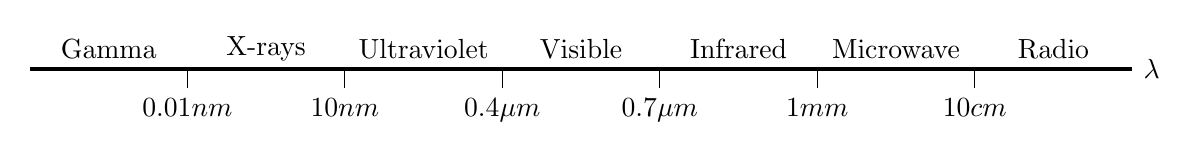
\begin{tikzpicture}[scale=0.5]
        % Spectrum lines
        \draw[ultra thick] (0,0) -> (28,0) node[right] {$\lambda$};

        % Wavelengths
        \foreach \w/\label in {4/$0.01nm$, 8/$10nm$, 12/$0.4\mu m$, 16/$0.7\mu m$, 20/$1mm$, 24/$10cm$}
            {
                \draw (\w,0) -- (\w,-0.5) node[below] {\label};
            }

        % Labels
        \foreach \w/\label in {2/Gamma, 6/X-rays, 10/Ultraviolet, 14/Visible, 18/Infrared, 22/Microwave, 26/Radio}
            {
                \node at (\w, 0.5) {\label};
            }

        % % Rainbow-colored band in the visible region (between 12 and 16)
        % \fill[red] (12,0) rectangle (12.8,0.2);
        % \fill[orange] (12.8,0) rectangle (13.6,0.2);
        % \fill[yellow] (13.6,0) rectangle (14.4,0.2);
        % \fill[green] (14.4,0) rectangle (15.2,0.2);
        % \fill[cyan] (15.2,0) rectangle (16,0.2);

    \end{tikzpicture}
    \caption{Spettro elettromagnetico}
\end{figure}

Con la conoscenza della lunghezza d'onda, è possibile calcolare la frequenza dell'onda elettromagnetica utilizzando la formula $f = \frac{c}{\lambda}$, in cui $c$ rappresenta la velocità della luce.
Un'importante porzione dello spettro è la luce visibile, con lunghezze d'onda comprese tra $400nm$ (viola) e $700nm$ (rosso).
Questa fascia visibile è cruciale per la percezione umana dei colori, spaziando attraverso l'interessante intervallo di colori che va dal viola al rosso.